\documentclass{standalone}
%\usepackage{tikz}
\usepackage{amsmath}
\usepackage{pgfplots}
%\usepackage{tikz-3dplot}

\pgfplotsset{compat=1.16}

\usetikzlibrary{arrows,intersections,math}

\begin{document}
	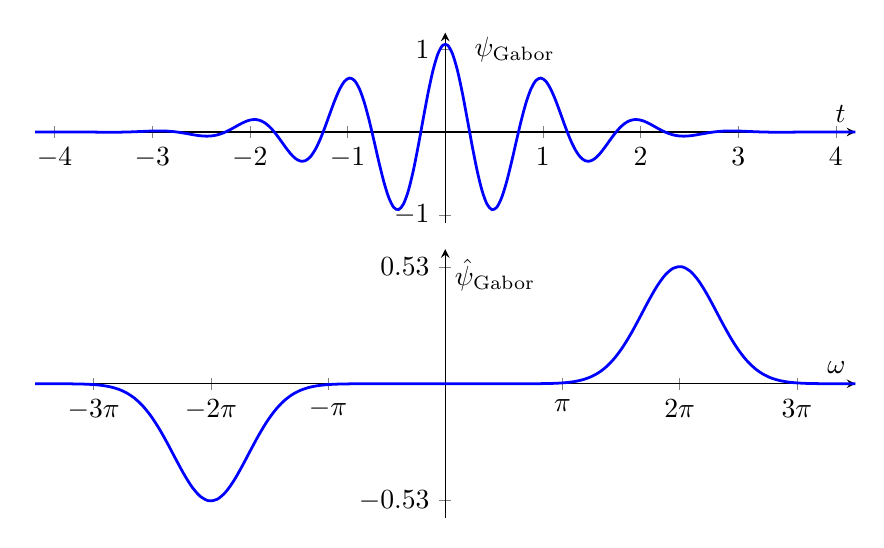
\begin{tikzpicture}
		\begin{scope}
			\begin{axis}[axis lines=middle, width=12cm, height=4cm,
				y label style={at={(axis cs:0.2, 1)},anchor=west},
				xmin=-4.2, xmax=4.2, ymin=-1.1, ymax=1.2,	xlabel=$t$,ylabel=$\psi_{\text{Gabor}}$]
				\addplot[domain=-5:5,samples=200, smooth, color=blue,line width=1pt] 
				{1.061*exp(-(\x^2)/2)*cos(360*\x)};
			\end{axis}
		\end{scope}
		\begin{scope}[yshift=-3.75cm]
			\begin{axis}[axis lines=middle, width=12cm, height=5cm,
				xmin={-3.5*pi}, xmax={3.5*pi}, ymin=-0.61, ymax=0.61,
				xlabel=$\omega$,ylabel=$\hat\psi_{\text{Gabor}}$,
				xtick={-3*pi, -2*pi, -pi, 0, pi, 2*pi, 3*pi},
				xticklabels={$-3\pi$,$-2\pi$,$-\pi$,,$\pi$,$2\pi$,$3\pi$},
				ytick={-0.53, 0.53}]
				\addplot[domain=-11:11,samples=100, smooth, color=blue,line width=1pt] 
				{0.751125544 / sqrt(2) * (exp(-((\x-2*pi)^2)/2) - exp(-((-\x-2*pi)^2)/2))};
			\end{axis}
		\end{scope}
	\end{tikzpicture}
\end{document}
